\subsection{Genus} % (fold)
\label{sec:genus}
Zaczniemy od starego twierdzenia, które klasyfikuje powierzchnie domknięte.

\begin{proposition}
    Każda powierzchnia domknięta jest członkiem jednej z dwóch nieskończonych rodzin:
    \begin{enumerate}[leftmargin=*]
        \itemsep0em
        \item sumą spójną $g \ge 0$ torusów,
        \item sumą spójną $k \ge 1$ rzeczywistych płaszczyzn rzutowych.
    \end{enumerate}
\end{proposition}

Elementy pierwszej rodziny są orientowalne.
Sferę traktujemy dla wygody jako sumę spójną $g = 0$ torusów.
Wtedy sumę spójną $g$ torusów możemy wyobrazić sobie jako sferę, do której doklejono $g$ uchwytów.

\begin{definition}[genus powierzchni]
    Ilość torusów nazywamy genusem powierzchni i oznaczamy literą $g$.
\end{definition}

Podobna charakteryzacja istnieje dla powierzchni z~brzegiem.
Każdy taki obiekt jest homeomorficzny z~sumą spójną $g$ torusów, w~których wydrążono pewną liczbę otworów: tyle, ile składowych spójności ma brzeg powierzchni.
W~przypadku powierzchni Seiferta mamy do czynienia z jednym otworem.

Dla wygody przypomnijmy jeszcze definicję klasycznego niezmiennika powierzchni:

\begin{definition}[charakterystyka Eulera]
    \index{charakterystyka Eulera}
    Niech $M$ będzie domkniętą powierzchnią orientowalną.
    Po striangulowaniu, składa się z $k_0$ wierzchołków, $k_1$ krawędzi oraz $k_2$ ścian.
    Wielkość
    \begin{equation}
        \chi = k_0 - k_1 + k_2
    \end{equation}
    jest niezmiennikiem powierzchni, zwanym zazwyczaj charakterystyką Eulera.
\end{definition}

Jeśli $M$ jest powierzchnią o genusie $g$ i $\mu$ składowych spójności brzegu, to $\chi = 2 - \mu - 2g$.
Nas interesują głównie powierzchnie Seiferta węzłów:

\begin{proposition}
    Niech $K$ będzie węzłem z~diagramem $D$.
    Wtedy $\chi(M_D) = d - b$, gdzie $b$ jest liczbą skrzyżowań $D$, zaś $d$ jest liczbą okręgów Seiferta.
\end{proposition}

\begin{proof}
    W~dowodzie faktu \ref{seifert_existence} widzieliśmy, że liczba skrzyżowań $b$ jest jednocześnie liczbą pasków doklejonych do dysków.
    Bezpośredni rachunek pokazuje, że wtedy $k_0 = 4b$, $k_1 = 6b$ oraz $k_2 = b+d$.
    Wynika stąd, że $\chi = 4b - 6b + b + d = d - b$.
\end{proof}

Reszta tej podsekcji nie jest wymagana do zrozumienia macierzy Seiferta, przyjrzymy się genusowi jako obiektowi ciekawemu samemu w sobie.

\begin{definition}[3-genus]
    Niech $K$ będzie węzłem.
    Minimalny genus spośród wszystkich powierzchni Seiferta węzła $K$ nazywamy 3-genusem i oznaczamy $g$.
\end{definition}

Znalezienie 3-genusu dowolnego węzła sprawia te same trudności, co wyznaczenie jego liczby gordyjskiej.
Dowolna powierzchnia Seiferta zadaje ograniczenie z góry.
Z dołu 3-genus można szacować przy użyciu wielomianu Alexandera:

\begin{proposition}
    Niech $K$ będzie węzłem.
    Wtedy $\operatorname{span} \Delta(t) \le 2g$.
\end{proposition}

\begin{proof}
    Załóżmy, że $F$ jest powierzchnią Seiferta węzła $K$ o genusie $g$.
    Wtedy macierz Seiferta powstała z $F$ jest rzędu $2g$, więc żaden ze składników jej wyznacznika nie może mieć stopnia większego niż $2g$.
    (To ma sens dopiero po przeczytaniu podsekcji ,,macierz Seiferta''!)
\end{proof}

\begin{proposition}
    Niech $K$ będzie węzłem.
    Wtedy $\operatorname{span} \Delta(t) = 2g$ wtedy i tylko wtedy, gdy $\det M \neq 0$.
    % Murasugi
\end{proposition}

To dolne ograniczenie jest realizowane przez pewną powierzchnię Seiferta dla każdego pierwszego węzła o~co najwyżej 11 skrzyżowaniach poza siedmioma wyjątkami: 11n42, 11n67, 11n97 ($g = 2$), 11n34, 11n45, 11n73 oraz 11n152 ($g=3$).
Jeżeli nie powoduje to nieporozumień, zamiast 3-genus można pisać po prostu genus.

Czy w definicji genusu można ograniczyć się do powierzchni Seiferta, które pochodzą od algorytmu Seiferta?
Niestety, poza pewnymi wyjątkami, nie.
Zanim przekonamy się, dlaczego tak jest, zdefiniujmy jeszcze dwa niezmienniki.

\begin{definition}[genus kanoniczny]
    Niech $K$ będzie węzłem.
    Minimalny genus spośród wszystkich powierzchni Seiferta węzła $K$, które pochodzą z~algorytmu Seiferta, nazywamy genusem klasycznym i~oznaczamy $g_c$.
\end{definition}

Pod koniec lat pięćdziesiątych Crowell i~Murasugi niezależnie zauważyli, że algorytm Seiferta zastosowany do alternującego diagramu zawsze daje powierzchnię o~minimalnej powierzchni.
Ich kombinatoryczne uzasadnienie było dość zawiłe, elementarny dowód podał Gabai w \cite{gabai86}.

Dubel trójlistnika ma genus równy $1$, ale algorytm Seiferta zastosowany wobec węzła produkuje powierzchnie o genusie co najmniej $3$, jak przewiduje ograniczenie znalezione przez Mortona w \cite{morton86} jako twierdzenie 2:

\begin{proposition}
    Niech $P(v, z)$ będzie wersją wielomianu HOMFLY spełniającą zależność
    \begin{equation}
        \frac 1v P_+ - vP_- = zP_0.
    \end{equation}
    Wtedy $M = \max \deg_z P(v, z) \le 2g_c$.
\end{proposition}

Nierówność Mortona jest równością dla wielu klas węzłów, w tym alternujących (Crowell, Murasugi), jednorodnych (które stanowią uogólnienie węzłów alternujących, Cromwell w \cite{cromwell89}), whiteheadowskich dubli węzłów dwumostowych (Nakamura w \cite{nakamura06}, Tripp w \cite{tripp02}) albo precli (Brittenham, Jensen w preprincie ,,Canonical genus and the Whitehead doubles of pretzel knots'').
Stojmenow pokazał, że staje się równością dla węzłów o co najwyżej 12 skrzyżowaniach i znalazł przykład węzła, dla którego jest ostra.

\begin{definition}[genus wolny]
    Niech $K$ będzie węzłem.
    Minimalny genus spośród powierzchni Seiferta węzła $K$, których dopełnienie w 3-sferze jest \emph{ciałem z rączkami} (handlebody, czyli ma wolną grupę podstawową), nazywamy genusem wolnym i~oznaczamy $g_f$.
\end{definition}

Dopełnienie powierzchni Seiferta jest zawsze handlebody, dlatego też mamy oczywiste nierówności $g \le g_f \le g_c$.
Morton w 1986 roku pokazał, że genus pewnych węzłów nie jest realizowany przez żaden diagram do którego stosuje się algorytm Seiferta, choćby $10_{165}$.
Patrz \cite{morton86}.
Moriah, matematyk izraelski, mniej więcej w tym samym czasie rozwiązał problem postawiony dekadę wcześniej przez Kirby'ego \cite{kirby78}: jak duża może być różnica $g_f - g$?

\begin{proposition}
    Niech $K$ będzie węzłem, $D_k(K)$ jego dublem Whiteheada z $k \neq 0$ skręceniami, zaś $B_n(K)$ to $n$-krotne nakrycie cykliczne sfery $S^3$ rozgałęzione nad węzłem $K$.
    Jeżeli ranga pierwszej grupy homologii $B_{|4k+1|}(K)$ wynosi $r$, to
    \begin{equation}
        g_f(D_k(K)) \ge \frac {2r-1} {|8k+2|}.
    \end{equation}
\end{proposition}

\begin{proof}
    Praca \cite{moriah87}.
    Dowód opiera się na chirurgii węzłów i splotów w sferze $S^3$.
\end{proof}

\begin{corollary}
    Niech $K$ bedzie sumą spójną $n$ trójlistników, połóżmy $k = -1$.
    Wtedy pierwsza grupa homologii ma rangę $r = 2n$ i~genus wolny jest nieograniczony
    \begin{equation}
        g_f(D_{-1}(3_1^n)) \ge \frac {4n-1} {6},
    \end{equation}
    podczas gdy zwykły genus to $g(D_{-1}(3_1^n)) = 1$.
\end{corollary}

\begin{proposition}
    \label{genus_one}
    Genus wykrywa niewęzły: $K$ jest niewęzłem wtedy i tylko wtedy, gdy $g(K) = 0$.
\end{proposition}

\begin{proof}
    Niech $K$ będzie węzłem o genusie $0$.
    Z~charakteryzacji powierzchni wynika, że jego powierzchnia Seiferta to suma spójna $0$ torusów, to znaczy kula z tyloma otworami, ile $K$ ma ogniw.
    Innymi słowy, powierzchnią Seiferta węzła $K$ jest dysk, którego brzeg stanowi niewęzeł.
    To pokazuje, że implikacja w lewo jest prawdziwa.

    Implikacja w prawo jest oczywista.
\end{proof}

\begin{proposition}
\label{genus_sum}
    Jeśli $J, K$ są węzłami, to $g (J \shrap K) = g(J) + g(K)$.
\end{proposition}

\begin{proof}
    Pokażemy najpierw, że $g(J \# K) \le g(J) + g(K)$.
    Wybierzmy powierzchnie Seiferta $M_J$ oraz $M_K$ dla $J$ oraz $K$ o~minimalnym genusie.
    Suma $J \shrap K$ powstaje z~$J$ oraz $K$, podobnie jest z~powierzchniami Seiferta:
    \[
        \begin{tikzpicture}[baseline=-0.65ex,scale=0.12]
        \draw[semithick,-Latex] (-7, -5) to (-5, -5) [in=right, out=right] to (-5, 5) to (-7, 5);
        \draw[semithick,Latex-] ( 7, -5) to ( 5, -5) [in=left, out=left] to ( 5, 5) to ( 7, 5);
        \node at (-5, 0) {$J$};
        \node at (5, 0) {$K$};
        \end{tikzpicture}
        \longrightarrow
        \begin{tikzpicture}[baseline=-0.65ex,scale=0.12]
        \draw[semithick,-Latex] (-7, -5) to (-5, -5) to [out=right, in=left] (-2, -2) -- (2, -2) to [out=right, in=left] (5, -5) to (7, -5);
        \draw[semithick,Latex-] (-7, 5) to (-5,  5) to [out=right, in=left] (-2,  2) -- (2,  2) to [out=right, in=left] (5,  5) to (7, 5);
        \node at (0, -5) {$J \# K$};
        \end{tikzpicture}
        \quad\quad
        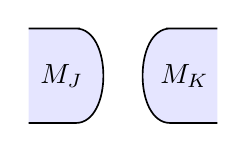
\begin{tikzpicture}[baseline=-0.65ex,scale=0.12]
        \draw[semithick,fill=blue!10!white] (-10, -5) to (-5, -5) [in=right, out=right] to (-5, 5) to (-10, 5);
        \draw[semithick,fill=blue!10!white] ( 10, -5) to ( 5, -5) [in=left, out=left] to ( 5, 5) to (10, 5);
        \node at (-6.5, 0) {$M_J$};
        \node at (6.5, 0) {$M_K$};
        \end{tikzpicture}
        \longrightarrow
        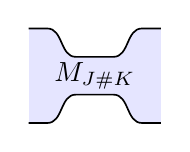
\begin{tikzpicture}[baseline=-0.65ex,scale=0.12]
        \fill[blue!10!white] (-7, -5) rectangle (7, 5);
        \draw[semithick,fill=white] (-7, -5) to (-5, -5) to [out=right, in=left] (-2, -2) -- (2, -2) to [out=right, in=left] (5, -5) to (7, -5);
        \draw[semithick,fill=white] (-7, 5) to (-5,  5) to [out=right, in=left] (-2,  2) -- (2,  2) to [out=right, in=left] (5,  5) to (7, 5);
        \node at (0, 0) {$M_{J \# K}$};
        \end{tikzpicture}
    \]

    Skoro $M_{J\#K}$ powstaje z~$M_J \sqcup M_K$ przez dołączenie paska do brzegu, mamy
    \[
        \chi(M_{J\#K}) = \chi(M_J \sqcup M_K) - 1 = \chi(M_J) + \chi(M_K)-1,
    \]
    a~przez to
    \[
        g(M_{J\#K}) = \frac{1-\chi(M_{J\#K})}{2} =
        \frac{1-\chi(M_{J})}{2} + \frac{1-\chi(M_{K})}{2}
        % = %g(M_J)+g(M_K)
        = g(J) + g(K).
    \]
    To kończy dowód pierwszej nierówności.
    Pokażemy jeszcze, że $g(J \# K) \ge g(J)+g(K)$.
    Zaczynamy od powierzchni Seiferta $M_{J\#K}$ dla $J\#K$ o~minimalnym genusie $g(M_{J\#K})$ równym $g(J\#K)$.
    Poprzez wykonanie chirurgii na powierzchni, możemy przyjąć specjalną postać jak w~poprzednim dowodzie:
    \[
        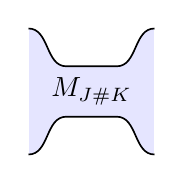
\begin{tikzpicture}[baseline=-0.65ex,scale=0.16]
            \fill[blue!10!white] (-5, -5) rectangle(5, 5);
        \draw[semithick,fill=white] (-5, -5) to [out=right, in=left] (-2, -2) -- (2, -2) to [out=right, in=left] (5, -5);
        \draw[semithick,fill=white] (-5,  5) to [out=right, in=left] (-2,  2) -- (2,  2) to [out=right, in=left] (5,  5);
            \node at (0, 0) {$M_{J \# K}$};
        \end{tikzpicture}
    \]

    Usunięcie paska daje powierzchnie Seiferta dla $M_J$ oraz $M_K$ takie, że
    \[
        g(M_J)+g(M_K)=g(M_{J\#K})=g(J\#K).
    \]
    Oznacza to, że $g(J)+g(K)\leqslant g(M_J)+g(M_K)=g(J\#K)$ i~tak naprawdę mamy równość.
\end{proof}

\begin{corollary}
\label{no_inverses}
    Jeśli suma spójna dwóch węzłów jest niewęzłem, to oba składniki także nim są.
\end{corollary}

Powrócimy teraz do węzłów pierwszych (definicja \ref{primeknot}).

\begin{proposition}
    Niech $K$ będzie węzłem.
    Jeśli $g(K) = 1$, to $K$ jest węzłem pierwszym.
\end{proposition}

\begin{proof}
    Załóżmy nie wprost, że $K = K_1 \# K_2$ jest sumą dwóch nietrywialnych węzłów.
    Z~faktu \ref{genus_sum} wynika wtedy, że $g(K) = g(K_1) + g(K_2)$.
    Zatem jeden z węzłów $K_1, K_2$ ma genus zero i jest trywialny, wbrew naszemu założeniu.
\end{proof}

Implikacja odwrotna jest fałszywa: pięciolistnik jest pierwszy, ale jego genus wynosi $2$.

\begin{proposition}
    Każdy węzeł można zapisać jako suma spójna pewnej liczby węzłów pierwszych (niewęzeł jest sumą pustej rodziny węzłów).
\end{proposition}

\begin{proof}
    Dowodzimy przez indukcję względem genusu $g(K)$.
    Przypadek bazowy $g(K) = 0$ jest oczywisty, gdyż wtedy $K$ to niewęzeł.
    Załóżmy więc, że fakt zachodzi dla węzłów $J$ genusu co najwyżej $n$.
    Niech $K$ będzie genusu $n + 1$.

    Jeśli $K$ jest pierwszy, nie ma czego dowodzić.
    W przeciwnym razie jest równoważny z~$J_1 \shrap J_2$, gdzie $J_1$ i~$J_2$ są nietrywialne.
    Mamy $g(J_1)+g(J_2)=g(K)$ oraz $g(J_1),g(J_2)\geqslant 1$.
    Zatem $g(J_1),g(J_2)\leqslant n$.
    Na mocy hipotezy indukcyjnej, $J_1$ oraz $J_2$ są równoważne sumom
    \[
        J_1 \cong K_1\#\cdots\# K_s,\qquad
        J_2 \cong K_{s+1}\#\cdots\# K_r,
    \]
    gdzie $K_i$ są pierwsze.
    Zatem $K$ jest równoważny z~$K_1\#\cdots\# K_r$, co kończy dowód.
\end{proof}

\begin{proposition}
\label{infty_primes}
    Istnieje nieskończenie wiele węzłów pierwszych.
\end{proposition}

\begin{proof}
    Pokażemy, że wszystkie węzły $(2n+2)_1$ są pierwsze, gdzie $n \ge 1$.
    Istotnie, algorytm Seiferta zastosowany do diagramu tego węzła wyprodukuje $2n+1$ okręgów.
    \[
        \begin{tikzpicture}[baseline=-0.65ex,scale=0.055]
        \begin{knot}[clip width=10, flip crossing/.list={1,4,5},end tolerance=1pt]
            \node at (0,10) {$\cdots$};
            \strand[semithick] (-30, -5) -- (-5, -5);
            \strand[semithick,-Latex]  (5, -5) -- (30, -5);
            \strand[semithick,Latex-]  (-30,-15) -- (-5,-15);
            \strand[semithick,Latex-]  (5,-15) -- (30,-15);

            \strand[semithick,domain=-90:90] plot ({7.5*cos(\x)-5}, {5*sin(\x)-10});
            \strand[semithick,domain=90:270] plot ({7.5*cos(\x)+5}, {5*sin(\x)-10});

            % zewnętrzne obręcze -- lewa strona
            \strand[semithick] (-30, 15) to [out=left, in=up]   (-45, 0);
            \strand[semithick] (-30,-15) to [out=left, in=down] (-45, 0);
            \strand[semithick] (-30,  5) to [out=left, in=up]   (-35, 0);
            \strand[semithick] (-30, -5) to [out=left, in=down] (-35, 0);

            % zewnętrzne obręcze -- prawastrona
            \strand[semithick] (30, 15) to [out=right, in=up]   (45,0);
            \strand[semithick] (30,-15) to [out=right, in=down] (45,0);
            \strand[semithick] (30,  5) to [out=right, in=up]   (35,0);
            \strand[semithick] (30, -5) to [out=right, in=down] (35,0);

            % jak w~drugim ruchu Reidemeistera - lewe
            \strand[semithick] (-30, 15) .. controls (-24, 15) and (-24,  5) .. (-20,  5);
            \strand[semithick] (-30,  5) .. controls (-24,  5) and (-24, 15) .. (-20, 15);
            \strand[semithick] (-10, 15) .. controls (-16, 15) and (-16,  5) .. (-20,  5);
            \strand[semithick] (-10,  5) .. controls (-16,  5) and (-16, 15) .. (-20, 15);

            % jak w~drugim ruchu Reidemeistera - prawe
            \strand[semithick] (30, 15) .. controls (24, 15) and (24,  5) .. (20,  5);
            \strand[semithick] (10, 15) .. controls (16, 15) and (16,  5) .. (20,  5);
            \strand[semithick] (30,  5) .. controls (24,  5) and (24, 15) .. (20, 15);
            \strand[semithick] (10,  5) .. controls (16,  5) and (16, 15) .. (20, 15);
        \end{knot}
        \end{tikzpicture}
        \longrightarrow
        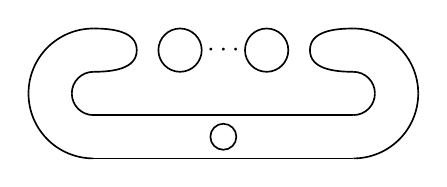
\begin{tikzpicture}[baseline=-0.65ex,scale=0.055]
            \node at (0,10) {$\cdots$};
            \draw[semithick] (-30,  -5) -- (30, -5);
            \draw[semithick] (-30, -15) -- (30,-15);

            \draw[semithick] (0,-10) circle (3);

                % zewnętrzne obręcze -- lewa strona
            \draw[semithick] (-30, 15) to [out=left, in=up]   (-45, 0);
            \draw[semithick] (-30,-15) to [out=left, in=down] (-45, 0);
            \draw[semithick] (-30,  5) to [out=left, in=up]   (-35, 0);
            \draw[semithick] (-30, -5) to [out=left, in=down] (-35, 0);

                % zewnętrzne obręcze -- prawastrona
            \draw[semithick] (30, 15) to [out=right, in=up]   (45,0);
            \draw[semithick] (30,-15) to [out=right, in=down] (45,0);
            \draw[semithick] (30,  5) to [out=right, in=up]   (35,0);
            \draw[semithick] (30, -5) to [out=right, in=down] (35,0);

            \draw[semithick] (-30, 15) to [out=right, in=up] (-20,10);
            \draw[semithick] (-30,  5) to [out=right, in=down] (-20,10);

            \draw[semithick] (30, 15) to [out=left, in=up] (20,10);
            \draw[semithick] (30,  5) to [out=left, in=down] (20,10);

            \draw[semithick] (-10, 10) circle (5);
            \draw[semithick] (10,  10) circle (5);
        \end{tikzpicture}
    \]
    Wynika stąd, że genus wynosi $\frac 12 (1 - (1+2n) + (2+2n)) = 1$, ponieważ wyznacznik ma wartość $4n+1$,
    węzły $2n+2)_1$ nie są trywialne i~są parami różne.
\end{proof}

\begin{proposition}
    Genus węzła $K$ jest związany z~wielomianem Alexandera oraz liczbą skrzyżowań:
    \[
        c(K) \ge 2 g(K) \ge \operatorname{Span}(\Delta_K(t)),
    \]
    przy czym (między innymi) dla węzłów o~co najwyżej 10 skrzyżowaniach mamy nawet równość po prawej stronie.
\end{proposition}

\index{homologia!Floera}
Wielomian Alexandera uogólnia się do (skomplikowanej) homologii Floera, pozwala ona dokładniej szacować genus węzła.

% Koniec podsekcji Genus

